\documentclass[10pt]{exam}
\usepackage[hon]{template-for-exam}
\usepackage{tikz}
\usetikzlibrary{shadings,decorations.pathmorphing,arrows.meta,patterns}

\tikzstyle{box}=[rounded corners,draw,minimum height=1cm,minimum width=1.5cm]


\title{Multi-Body Practice Problems}
\author{Rohrbach}
\date{\today}

\begin{document}
\maketitle


\noindent
For each situation, (a) Draw a free-body diagram for \emph{each} box; (b) Calculate the acceleration of the system; (c) Calculate the tension of the cord connecting the boxes.

\begin{questions}

\question

Two boxes have masses $m_1=20$ kg and $m_2=10$ kg and are sitting on a frictionless surface connected by a massless cord. They are pulled with an applied force of $F=50$ N.

\vspace{2em}

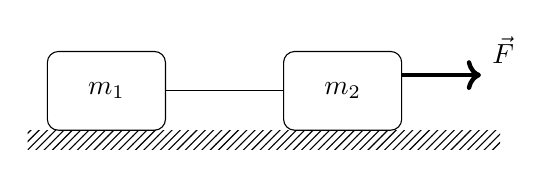
\begin{tikzpicture}
  \node[box] (one) at (0,0) {$m_1$};
  \node[box] (two) at (3,0) {$m_2$};
  \draw (one.east) -- (two.west);
  \draw[->,ultra thick] (two.east) ++(0,0.2) -- +(1,0) node[anchor=south west] {$\vec{F}$};
  \fill[pattern=north east lines] (-1,-0.5) rectangle ++(6,-0.25);
\end{tikzpicture}


\vs[2]

\question
Two masses are attached by a string that hangs over a frictionless pulley.  (This is known as an \emph{Atwood Machine})

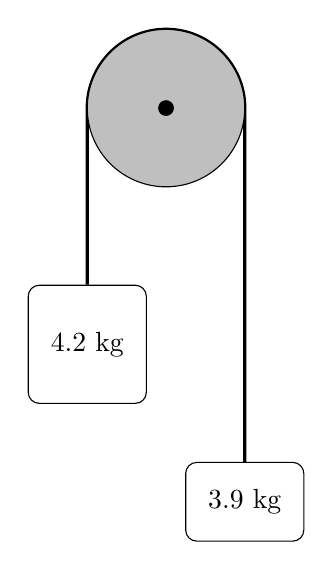
\begin{tikzpicture}
  \node[box,minimum height=1.5cm] (one) at (-1,0) {4.2 kg};
  \node[box] (two) at (1,-2) {3.9 kg};
  \draw[very thick] (one.north) -- (-1,3) 
    arc (180:0:1) -- (two.north);
  \draw[fill=gray!50] (0,3) circle[radius=1];
  \fill (0,3) circle[radius=0.1];
\end{tikzpicture}

\vs

\pagebreak


\question
We now have what is called a \emph{Modified Atwood Machine}. Again, the surface is frictionless.

\vspace{2em}

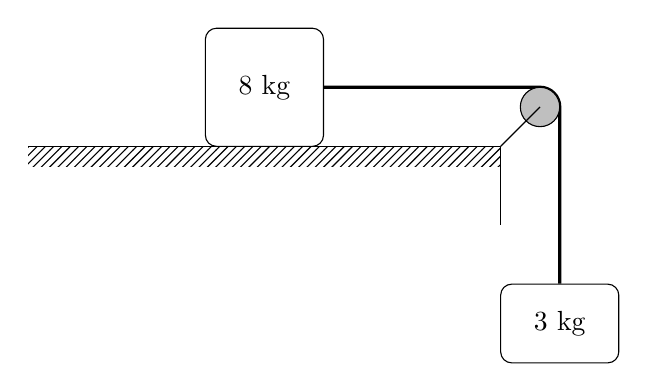
\begin{tikzpicture}
  \node[box,minimum width=1.5cm,minimum height=1.5cm] (one) at (0,0) {8 kg};
  \node[box] (two) at (3.75,-3) {3 kg};
  \draw[very thick] (one.east) -- (3.5,0) arc (90:0:0.25) -- (two);
  \fill[pattern=north east lines] (-3,-0.75) rectangle
    ++(6,-0.25);
  \draw (-3,-.75) -- 
    ++(6,0) coordinate (edge) -- 
    ++(0,-1);
  \draw[fill=gray!50] (edge) -- (3.5,-0.25) circle (0.25);
\end{tikzpicture}

\vs


\question \textbf{Challenge!}. For this problem, calculate the tension on each cord and the acceleration of the system.


\vspace{2em}

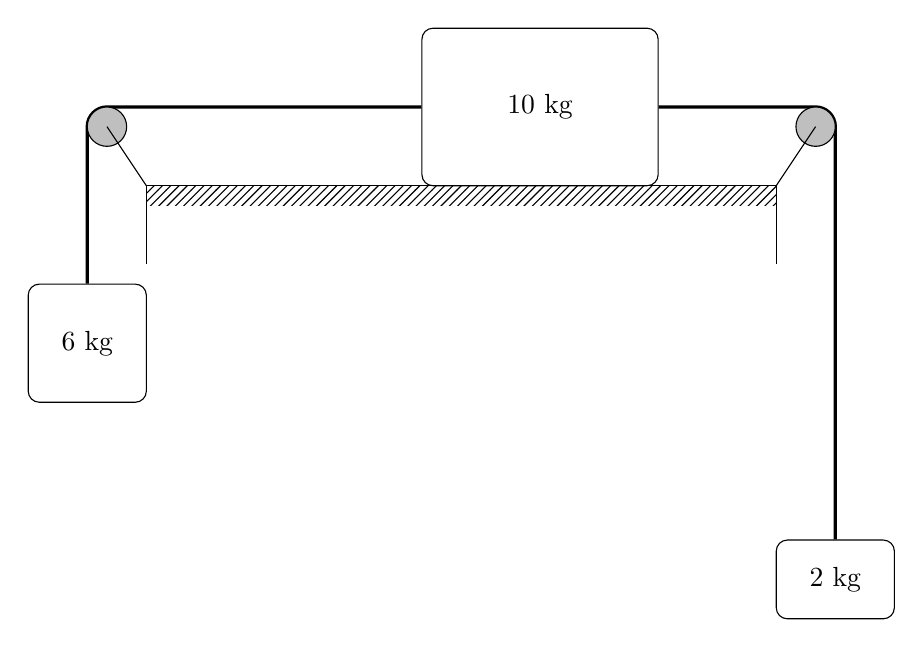
\begin{tikzpicture}
  \node[box,minimum width=3cm,minimum height=2cm] (one) at (0,0) {10 kg};
  \node[box] (two) at (3.75,-6) {2 kg};
  \node[box,minimum height=1.5cm] (three) at (-5.75,-3) {6 kg};
  \draw[very thick] (one.east) -- (3.5,0) arc (90:0:0.25) -- (two);
  \draw[very thick] (one.west) -- (-5.5,0) arc (90:180:0.25) -- (three);
  \fill[pattern=north east lines] (-5,-1) rectangle
    ++(8,-0.25);
  \draw (-5,-1) --
    ++(8  ,0) coordinate (edge) -- 
    ++(0,-1);
  \draw[fill=gray!50] (edge) -- (3.5,-0.25) circle (0.25);
  \draw (-5,-1) coordinate (edge 2) -- ++(0,-1);
  \draw[fill=gray!50]  (edge 2) -- (-5.5,-0.25) circle (0.25);


\end{tikzpicture}


  
\end{questions}

\end{document}